\documentclass[5pt]{article}
\usepackage{multicol,multirow}
\usepackage{graphicx} % Required for inserting images
\usepackage[margin=0.75cm]{geometry}
\usepackage{xcolor}
\usepackage{amsmath,esint}
\usepackage{mathtools}
\usepackage{relsize}
\usepackage{mathtools}
\usepackage{nccmath}


\usepackage{empheq}
\usepackage{amsfonts}

\usepackage{tkz-euclide}
\usepackage{tikz}

\definecolor{LightGray}{gray}{0.9}

\usepackage{minted}

\newenvironment{amatrix}[1]{%
  \left[\begin{array}{@{}*{#1}{c}|c@{}}
}{%
  \end{array}\right]
}

\DeclarePairedDelimiter\abs{\lvert}{\rvert}%
\DeclarePairedDelimiter\norm{\lVert}{\rVert}%

\makeatletter
\let\oldabs\abs
\def\abs{\@ifstar{\oldabs}{\oldabs*}}

\newcommand{\tr}[3]{
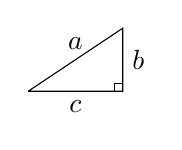
\begin{tikzpicture}[scale=0.40]
    \coordinate [] (A) at (-1.5cm,-1.cm);
    \coordinate [] (C) at (1.5cm,-1.0cm);
    \coordinate [] (B) at (1.5cm,1.0cm);
    \draw (A) -- node[above] {$a$} (B) -- node[right] {$b$} (C) -- node[below] {$c$} (A);
    \draw (1.25cm,-1.0cm) rectangle (1.5cm,-0.75cm);
\end{tikzpicture}
}


\begin{document}


\begin{center}
     \Large{\textbf{Linear Algebra}}\\
     \small{Class: ...}\hfill\small{\textcopyright Maximilien Notz \the\year{}}
     \noindent\rule{20.2cm}{0.4pt}
\end{center}


\begin{multicols}{2}
\setcounter{secnumdepth}{0}


\subsection{Definition}
\begin{tabular}{ll}
    Linear Functions & All terms are of  degree 0 or 1. \\
                   & A solution of a system of linear \\ 
                   & equation is set of points that makes \\
                   & the equation system true. \\
     Consistent    & lin. systems is consistent if either 1 or $\infty$ \\
                   & solutions exist else inconsistent.\\
     Conist
\end{tabular}


\subsection{Coefficient Matrix}
\begin{equation}
\centering
\left\{\begin{split}
A_1x_1+A_2x_2+A_3x_3=\alpha \\
B_1x_1+B_2x_2+B_3x_3=\beta \\
C_1x_1+C_2x_2+C_3x_3=\gamma \\
\end{split}\right.
\Leftrightarrow
\begin{bmatrix}
    A_1 & A_2 & A_3\\
    B_1 & B_2 & B_3\\
    C_1 & C_2 & C_3\\
\end{bmatrix}
\end{equation}


\subsection{Augmented Matrix}
\begin{equation}
\left\{\begin{split}
A_1x_1+A_2x_2+A_3x_3=\alpha \\
B_1x_1+B_2x_2+B_3x_3=\beta \\
C_1x_1+C_2x_2+C_3x_3=\gamma \\
\end{split}\right.
\Leftrightarrow
\begin{amatrix}{3}
    A_1 & A_2 & A_3 & \alpha \\
    B_1 & B_2 & B_3 & \beta \\
    C_1 & C_2 & C_3 & \gamma \\
 \end{amatrix}
\end{equation}


\subsection{Row-Equivalence}
Two matrce are row-equivalent if there is a sequence of \textbf{EROS} that transforms one into the other.


\subsection{Elementary Row Operations (EROS)}
1. \textbf{[Replacement]} Replace one row by sum of itself. \\
2. \textbf{[Interchange]} Swap position of 2 rows. \\
3. \textbf{[Scaling]} Multiply all entries in row by non-zero constant. \\


\subsection{Echelon Form (ef)}
1. All non-zero rows are above any rows of all-zero. \\
2. Each leading entry of a row is in a column to the right of the roe above it. \\
3. All entries in a column below a leading entry are 0. \\


\subsection{Reduced Row Echelon Form (rref)}
1. As to be in echelon form. \\
2. Leading entry in each row is 1. \\
3. Each leading 1 is the only non-zero entry in its column. \\


\subsection{Theorems}
\newtheorem{theorem}{Theorem}
\newtheorem{properties}{Properties}
\begin{theorem}
Every matrix is row equivalent to a unique row echelon form.
\end{theorem}

\begin{theorem}
Every matrix is row equivalent to a unique row echelon form.
\end{theorem}


\section{Orthogonality and Diagonalization}
\subsection{Definition}
\begin{tabular}{ll}
  Inner Product       & $\vec{v}\cdot\vec{u}=\vec{v}^T\vec{u}=u_1v_1 + ... + u_nv_n$\\
                      & \footnotesize{(Also called dot product or scalar product)}\\
  Length of $\vec{x}$ & $||\vec{x}||=\sqrt{\vec{x}\cdot\vec{x}}=\sqrt{x^2_1+...+x^2_n}$\\
                      & \footnotesize{(Also called Norm or Magnitude)}\\
  Unit vectore        & A vector with $||\vec{x}||=1$
  
\end{tabular}

\subsection{Theorems}
\begin{properties}
  Let $\vec{u},\vec{v},\vec{w} \in \mathbb{R}^n$ and $c\in \mathbb{R}^n$
  \begin{itemize}
    \item $\vec{u}\cdot\vec{v}=\vec{v}\cdot\vec{u}$ 
    \item $(\vec{u}+\vec{v})\cdot \vec{w}=\vec{u}\cdot\vec{w}+\vec{v}\cdot \vec{w}$
    \item $(c\vec{u})\cdot \vec{v}=c(\vec{u}\cdot \vec{v})=(c\vec{v})\cdot \vec{u}$
    \item $\vec{u}\cdot \vec{u}=u_1^2+...+u^2_n\geq 0$
  \end{itemize}
\end{properties}

\end{multicols}
\end{document}